% IEEE standard conference template; to be used with:
%   spconf.sty  - LaTeX style file, and
%   IEEEbib.bst - IEEE bibliography style file.
% --------------------------------------------------------------------------

\documentclass[letterpaper]{article}
\usepackage{spconf,amsmath,amssymb,graphicx}
\usepackage{minted}
\usepackage{listings}
\usepackage{float}
\usepackage{subcaption}
\usepackage{verbatim}
\usepackage{caption}
\usepackage{subcaption}
\usepackage{hyperref}

\urlstyle{same}

\captionsetup{compatibility=false}
% Example definitions.
% --------------------
% nice symbols for real and complex numbers
\newcommand{\R}[0]{\mathbb{R}}
\newcommand{\C}[0]{\mathbb{C}}
\newcommand{\figref}[1]{\textit{figure \ref{#1}}}
\newcommand{\secref}[1]{\textit{section \ref{#1}}}
\newcommand{\mypar}[1]{{\bf #1.}}

% Title.
% ------
\title{Multi-core Parallel Ripple Search}
%
% Single address.
% ---------------
\name{Gavin Gray, Lorenzo Liso, Dario Mylonopoulos, \\ \emph{Ishaan Shamanna, Lucas Weitzendorf} }

\address{DPHPC Project Report HS21 \\ ETH Z\"urich\\Z\"urich, Switzerland}


\begin{document}

%
\maketitle
%

\begin{abstract}
Pathfinding is a heavily researched area of Computer Science where sequential algorithms have since long been the focus.
Commonly used algorithms are difficult to parallelize effectively and therefore fail to take full advantage of modern computer architectures.
This report documents an implementation of parallel ripple search and demonstrates its significant performance increase compared to sequential references.
Parallel ripple search is an efficient approach to parallel pathfinding for a single source-target pair and provides opportunities for even further optimization to future problems.
\end{abstract}

\section{Introduction}\label{sec:intro}
From navigation to video games \cite{GMaps}, single source-target pair pathfinding can be found at the heart of many systems. 
As problem sizes increase, it becomes difficult for serial algorithms to achieve acceptable latency. 
Parallel ripple search, as proposed by Bidarra et al. \cite{PRS}, aims to leverage modern multi-core architectures by effectively parallelizing the problem and dividing the search space across threads. 
This report will focus on implementing and benchmarking parallel ripple search to investigate its advantages and disadvantages over other pathfinding algorithms.
The source code of this implementation can be found on GitHub
\footnote{The full source code can be found at \url{https://github.com/lweitzendorf/parallel-ripple-search}}
under the MIT license.

\section{Related Work}\label{sec:relatedwork}
Pathfinding is a very old problem and many good serial implementations exist.
Important serial algorithms, such as Dijkstra and A*, don't always translate well to a multi-core setting. 
Algorithms that sacrifice path length for performance gains such as fringe search \cite{Fringe} show more promise in this regard.

\mypar{A*} 
The natural serial algorithm to pick for pathfinding is A* \cite{A*}, its use of a heuristic cost function $h(n)$ that estimates the cost from vertex $n$ to the target, makes extending the explored space simple and efficient. 
Common implementations keep a \textit{min-heap} of open vertices, choosing a path that optimizes the cost function $f(n) = g(n) + h(n)$, where $g(n)$ is the actual cost from source to vertex $n$.
This allows A* to explore the unvisited neighboring vertices closest to the target in each iteration, finding the best path in an efficient manner.

\mypar{Parallelized A*} 
Many attempts have been made to parallelize A*. However, due to its reliance on a sorted data structure, there is no efficient way to distribute work among cores. In fact, handling concurrent updates to this structure becomes such a bottleneck that a serial version of A* often outperforms its various parallelizations \cite{parallel-astar}. 

\mypar{Fringe} 
At its core, fringe search is very similar to A*; it merely sacrifices optimality for runtime \cite{Fringe}.
Instead of keeping a sorted data structure that needs to have invariants re-established when the mininum element is removed, fringe simply keeps a list of all vertices in the search boundary. 
The algorithm then explores those that have better heuristics than a certain threshold value.
This saves computational time for exploration by removing the necessity to keep a data structure sorted but still expands the search space in an informed manner.

\mypar{Distributed Fringe} 
A parallel version of fringe search was proposed by S. Brand \cite{distributed-fringe}. As the vertices to be explored are unsorted, work can be distributed over multiple cores. 
However, the author showed many shortcomings of this approach. In particular, the fact that work is typically not distributed evenly across cores. 
In fact, the heuristic restricts the search boundary only in the most promising direction, which can only be followed by a single core at a time.

\mypar{Bidirectional} 
To make use of at least \textit{two} CPU cores when generating a path, one can start any serial algorithm twice: one search from the source towards the target, the other in reverse.
Typically, A* is used for this and the path is recreated from wherever the two searches meet. This is trivially parallelizable and referred to as parallel bidirectional search \cite{PRS}. The obvious shortcoming of this algorithm is that modern architectures have far more than two available cores and the scalability requirement is not met.

\section{Parallel Ripple Search}\label{sec:ripplesearch}
The following version of \textit{parallel ripple search} (PRS) is slightly modified from the one proposed by Bidarra et al. \cite{PRS}.
At a high level, the algorithm avoids the shortcomings of the parallel approaches discussed above by dividing the search space evenly across threads and removing dependency on a shared structure of open vertices.

This is done by isolating individual searches to a subsection of the graph and then reconstructing the solution in a divide-and-conquer fashion.

\mypar{Overview} 
At its core,  PRS can be broken down into four distinct phases which will be referred to as: high-level graph generation, space flooding, path refinement, and reconstruction. 
This implementation splits the work between a \textit{coordinator thread} and \textit{search threads}.
The coordinator is a separate thread which guides and schedules the work done by the search threads.
The coordinator also facilitates messages passed, thus removing intra-search-thread communication outside of synchronizing on shared memory.
A diagram depicting the flow of data between the coordinator and each search thread can be found in \figref{fig:high_level_flow}.
The decision was made to use a fringe search for each individual search thread in this implementation. However, different searches could be used, which would also affect the overall quality and performance of the algorithm.

\begin{figure}[H]
    \centering
    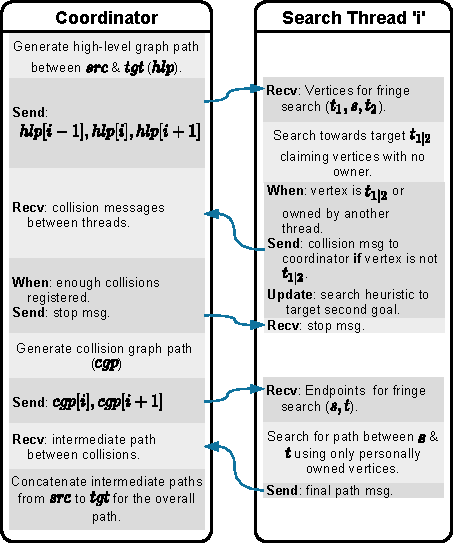
\includegraphics[width=.75\linewidth]{img/prs-flow-2.pdf}
    \caption{High-level logic and flow between the coordinator and search threads from PRS implementation.}
    \label{fig:high_level_flow}
\end{figure}

\mypar{High-Level Graph Generation}
The high-level graph is a coarse representation of the underlying search space and is used further to approximate where individual search threads should start from.
The high-level graph generation is an essential step in order to have distributed work amongst processes. 
A good high-level graph approximates the entire search space while reflecting expected vertex adjacencies. 
However, it should also be small, with a path length from source to target approximately equal to the number of available search threads.
Constructing a good high-level graph is a difficult task. However, this luckily only needs to happen once per graph. 
Therefore, once a high-level graph is generated, it can be stored and reused for subsequent path searches.
In this project, pathfinding was kept general enough to be applicable to any graph with vertex position information, making high-level graph generation more difficult. An applied use of PRS, where underlying graph characteristics are known a priori, could easily optimize this step. 
Further discussion on the details of the high-level graph generation and subsequently, the high-level path, will be deferred until \secref{sec:implementation}.

\begin{figure}[H]
    \centering
    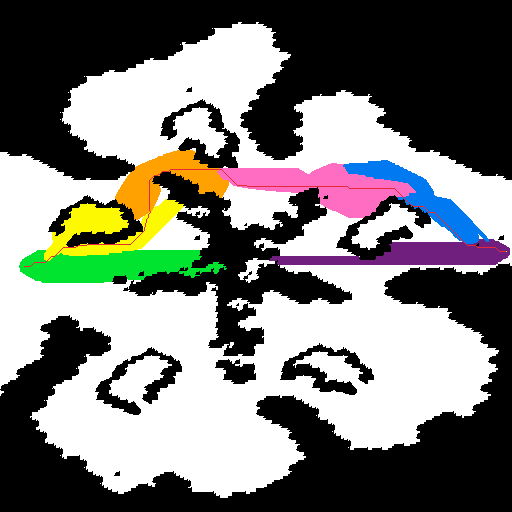
\includegraphics[width=.5\linewidth]{img/ripple.png}
    \caption{Final colored graph cache of PRS with 6 search threads with reconstructed path traced in red.}
    \label{fig:ripple_example}
\end{figure}

\mypar{Space Flooding} \label{par:space-flooding} 
In this initial search phase, a search thread $tid_i$ is started from each vertex of the high-level path, given two search targets, the source node of $tid_{i - 1}$ and $tid_{i + 1}$. 
These threads use a fringe search to explore the space around them, claiming vertices in cache as they are traversed, continuing until they reach the search space of a nearby thread or the current search target. 
After such a collision, the threads will change heuristic and start searching in the opposite direction, similar to bidirectional search. 
Two special cases are the search threads started from the global source and target vertices, which only have one neighboring thread, and thus will not perform a bidirectional search. During the exploration of the search space, the search threads communicate with the coordinator thread by informing it of encountered collisions between thread spaces. The coordinator thread registers the location and thread IDs of a collision and continuously tries to create a path via collision points from the source to target of the overall search. When such a path is found, the coordinator will halt the space flooding. An example of how threads flood the space can be seen in \figref{fig:ripple_example}.

\mypar{Path Refinement} 
After the threads have flooded the space and a path from the source to target has been found, each search thread will use a fringe search to find the shortest path between two collision points using only their region of claimed vertices. Under the assumption that the collision points between search threads lie close to an optimal path, restricting the search space of a thread in this manner will improve performance and have few adverse effects on the quality of the resulting path.

\mypar{Reconstruction} 
Once a path between each collision point is found, a path between the global source and target vertices can be reconstructed. 
The coordinator thread will simply concatenate the intermediate paths returned by each search thread in the order of the collision path.


\section{Implementation}\label{sec:implementation}
Now that the high-level algorithm has been described, an in-depth view of implementation details for PRS on a shared memory architecture can be provided. This is accompanied by a narrative of strategies that proved to be successful and others which were observed to have little, or negative effects on the system.

\mypar{High-Level Graph Generation} 
With our high-level graph, we tried to be as general as possible without exploiting the domain of video game maps (e.g hand-picking and connecting important points in the map). However, the underlying graph was fixed to a two-dimensional space to reduce complexity. The generation algorithm takes place in a few steps. 
First, a $64 \times 64$ mesh is overlaid on the graph's 2D space. 
This mesh is then reduced by picking only the points which lie in the actual graph and discarding the others.
Second, the remaining mesh vertices are connected to their eight respective neighbors, if they exist, using the same cost as that from the underlying graph.
If a neighbor does not exist, the vertex is connected to the next closest mesh vertex with a cost equal to the Euclidean distance multiplied by a large constant.
This strategy imposes a large penalty on paths through the high-level graph that  pass through walls or otherwise don't exist. 
It also is simple enough that generating this high-level graph does not incur a large overhead cost for PRS.
Lastly, mesh vertices are selected which are the closest to the source and target search vertices. An A* search is then used to find the shortest path through the high-level graph which has been previously referred to as the \textit{high-level path}. 
One desired property of the high-level path is that it is equal in length to the number of search threads. 
For the purpose of balancing work amongst threads, having equidistant starting points for the search threads is crucial.
Therefore, a high-level path is initially created at full grid resolution, which is then reduced in length to match the number of desired search threads while maintaining equidistant spacing.

\begin{figure}[H]
	\centering
	
	\captionsetup[subfigure]{labelformat=empty}
	\subfloat{
		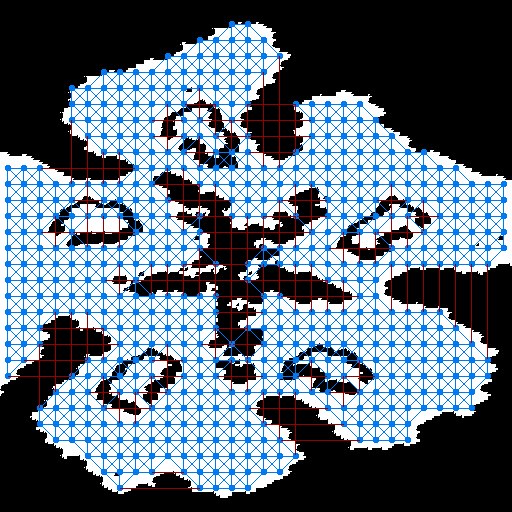
\includegraphics[width=0.22\textwidth]{img/high_path.png}
	}
	\hfill
	\subfloat{
		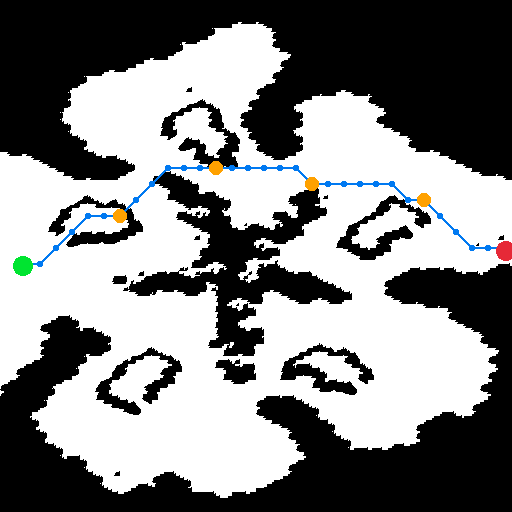
\includegraphics[width=0.22\textwidth]{img/high_graph.png}
	}
	\caption{(Left) a 32x32 mesh laid on top the \textit{StarCraft Predators} map with heavily weighted edges shown in red. (Right) The high-level path and thread starting points constructed from the left mesh, the same used for \figref{fig:ripple_example}.} 
	\label{fig:high}
\end{figure}

\mypar{Shared Lock-Free Cache}
A common technique used in many pathfinding algorithm implementations is storing some state information in the vertices themselves. 
This information typically is comprised of traversal data such as predecessor vertices, intermediate costs, etc.
For PRS specifically, each vertex can be owned by one thread and the decision was made to shift all of this runtime information into a cache structure shared between threads.
This implementation scales well, however, access to the cache needs to be synchronized to avoid data races on vertex acquisition.
To protect reads and writes, threads acquire a vertex by using an atomic \textit{compare and swap} operation to mark the vertex with its unique thread identifier and the predecessor vertex packed into a 64 bit integer. In intermediate solutions, private caches were used to try and reduce the need for synchronization. However, the additional memory initialization nullified any performance improvements in this regard. Similarly, using a single cache for both search phases requires the use of a validity tag, which needs to be checked with every access. In an attempt to remedy this, the cache was duplicated with one copy for each phase. However, this slight improvement was also offset by the increased memory initialization.
A note on implementation: special care was taken when implementing ownership of vertices in the cache. 
It took several design iterations until race conditions were no longer an issue. This especially manifested itself with setting the predecessor pointers when search threads were started too close to one another.
One more reason why load balancing of work between threads is important.

\mypar{Handling Collisions} 
A collision is detected whenever a thread fails to acquire a vertex because it's already owned by another thread.
When this happens, information about the collision, such as the threads involved, the vertex where it happened, and its predecessor, needs to be sent to a designated coordinator thread managing the overall search progress.
Search threads communicate with the coordinator via a message passing interface implemented over concurrent queues \cite{oneTBB}.
As previously mentioned, communication happens between the coordinator and search threads, but not between two search threads, thus reducing communication overhead and balancing work properly.
This implementation decision diverges from previous literature. It was observed that if a search thread handled communication, as is suggested in previous work, the \textit{refinement} phase of PRS took longer than necessary due to large differences in the size of a thread's search space.

\mypar{Vectorization}
To take advantage of vector instructions of modern x64 processors, an attempt was made to implement the core loop of fringe search using AVX512 intrisnics. 
In particular, the loading of neighboring vertices and storing the updated information in the cache was vectorized using scatter and gather operations.
Furthermore, newly-visited vertices and vertices that have their associated cost reduced by the discovery of a less expensive path, have to be inserted in the list of currently considered vertices.
The implementation of fringe search proposed by Bj\"ornsson et al. \cite{Fringe} stores the current nodes in a doubly linked list.
In this implementation, a linear array was used to take advantage of AVX512 \verb|vpcompress| instructions for appending elements efficiently without falling back to scalar code.
We measured the execution time of fringe search with a doubly-linked list and with a linear array. For the latter, both scalar and vectorized code were measured.
In measurements, using a linear array resulted in a noticeable speedup compared to the doubly linked list implementation. However, vectorized code did not provide any improvement over the scalar version.
We conjecture that this is due to the high cost of the scatter and gather operations combined with little arithmetic work.   
Therefore, in all further discussions of performance, the usage of ``vectorized'' will refer to the implementation using a linear array and not to the usage of vector instructions.


\section{Benchmark Environment}\label{sec:experimental}
\mypar{Data Set and Scenarios} 
In order to benchmark this ripple search implementation with the aim of making results comparable to future and past papers, it was decided to use the public data set proposed in \cite{6194296}, comprised of different grid-based video game maps. 
In particular, testing was conducted on the maps of \emph{StarCraft (SC)}, a popular real-time strategy game published in 1998 by Blizzard Entertainment, Inc. The repository contains 75 maps, most of which span at least $512 \times 512$ vertices.
For each map, multiple scenarios are tested, where a scenario is described by two $(x, y)$ coordinates representing the source and target respectively.
The total number of scenarios in the data set is $211,390$ and optimal path lengths range from $1$ to $2,155$.

\mypar{System Specifications}
All benchmarks were run on Windows Subsytem for Linux (5.10.16.3-microsoft-standard-WSL2, Ubuntu 20.04.3 LTS, Windows 11 Pro 22000.376).
The system was equipped with an AMD Ryzen 5900X 12-core CPU @ 3.70 GHz with 2x 16GB DDR4-3600 RAM and the project was compiled using CMake 3.16.3 and g++ 9.3.0 with the -O3 optimization flag. 
Runtime measurements were taken with LibSciBench \cite{libscibench} version 0.2.2. Further third-party libraries used: Boost 1.78.0 \cite{boost}, oneTBB 2021.5.0 \cite{oneTBB}, and GLM 0.9.9.8 \cite{glm}.

\mypar{Reference Implementations}
As a reference point for performance on the benchmark maps, PRS was compared with several sequential algorithms.
Specifically, 
\lstinline{astar_search} from the Boost C++ library
%% Footnote
\footnote{It should be noted that Boost's \lstinline{astar_search} works on generalized graphs as the underlying structure rather than a grid which is utilized by the other sequential references.},
%%%
a custom A* implementation,
the custom \textit{fringe} implementation as used in the search threads of PRS,
similarly the \textit{fringe vec} fringe search variant using a linear vector instead of a doubly linked list.
Lastly, an A* implementation adapted from \cite{heyesAStar} was also tested, this being used in several real-time applications. However, while highly optimized for smaller paths, the algorithm scaled too poorly to be included in the full benchmark run.

\mypar{Configuration}
The number of data points necessary was estimated from a limited test run over a subset of the benchmark suite, using confidence intervals on a t-distribution, as described by Hoefler et al. \cite{hoefler2015}. This resulted in an estimated minimum of $30$ runs per scenario to achieve a median variance within less than $5\%$ of the mean runtime with $99\%$ confidence.


\section{Results}
In this section, the results of the benchmark runs will be analyzed and presented.
When discussing the number of threads $N$, this number will include the coordinator thread except where specified.
It was previously discussed that PRS requires each search thread $tid_i$, where $i > 2$ to do two iterations of fringe search. 
In other words, the amount of work doubles once the algorithm is run with more than three threads. 
Taking this into account, the expected speedup of PRS is calculated as follows:

\begin{align*}
    & work = 
    \begin{cases} 
        1 & N \leq 3 \\
        2 & N > 3
    \end{cases} 
    & speedup = \frac{N-1}{work}
\end{align*}

\noindent where $N$ is the total number of threads including the coordination thread. This can be compared to the average runtime as shown in \figref{fig:runtime}. Expected runtime is defined as the quotient of sequential runtime and expected speedup.

\begin{figure}[H]
    \centering
    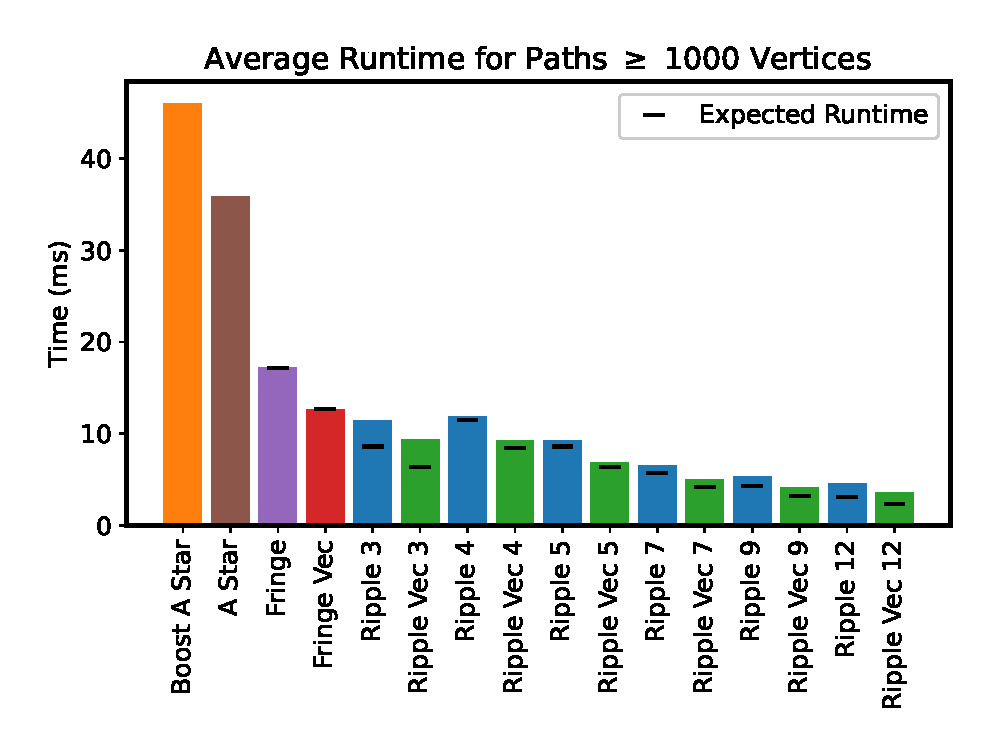
\includegraphics[width=\linewidth]{img/runtime.eps}
    \caption{Comparative runtime performance on large paths for all relevant algorithm implementations. The expected runtime is based on the corresponding sequential algorithm performance.}
    \label{fig:runtime}
\end{figure}

\noindent For sufficiently large graphs, PRS achieves almost linear speedup up to approximately 8 search threads compared to sequential fringe search. 
The vectorized versions of both fringe search and PRS outperform their counterpart at any given thread count, and as is clear, both PRS and fringe search outperform A*. 
The likely culprit of Boost's \linebreak\lstinline{astar_search} performance deficit is its underlying graph representation. Using a generalized graph seemed to be slightly slower on dense maps and significantly faster on sparse ones, however, as the benchmarks maps are mostly dense, the performance delta to our A* implementation can be easily explained.

\begin{figure}[H]
    \centering
    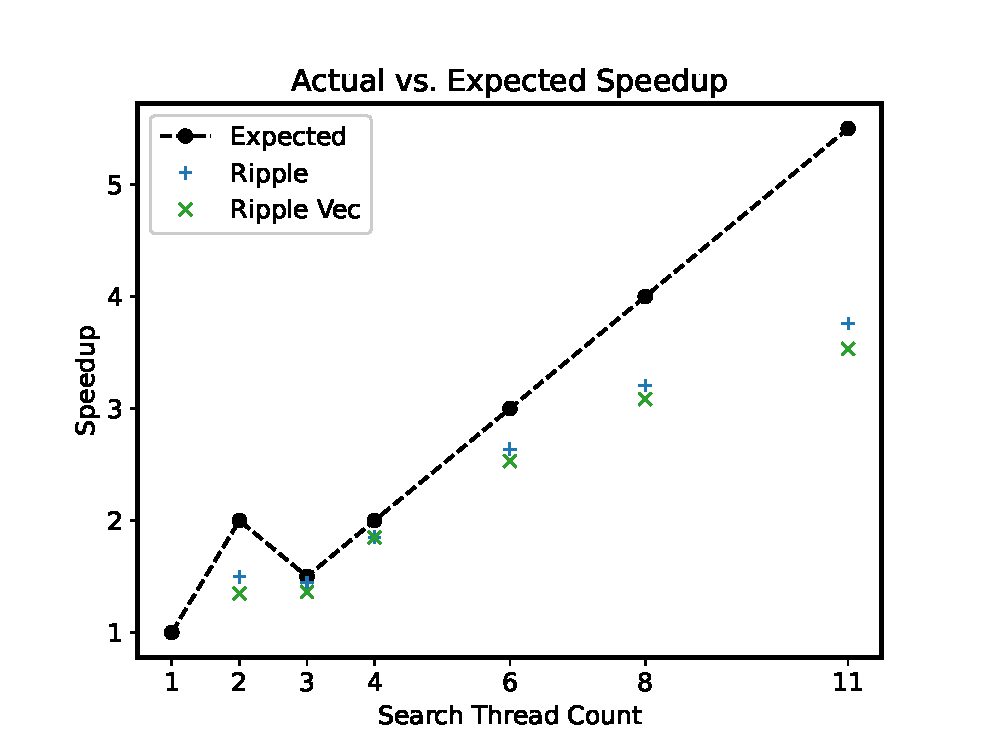
\includegraphics[width=\linewidth]{img/speedup.eps}
    \caption{Achieved speedup compared to the baseline fringe search for increasingly more \textit{search threads} over all benchmark scenarios.}
    \label{fig:speedup}
\end{figure}

\noindent All algorithm configurations are tested on the same set of benchmarks, thus relying on strong scaling. 
Observing \figref{fig:speedup}, PRS misses the mark with two search threads, where the initialization and coordination overhead seems to outweigh any improvements in search time.
In limited testing with randomly generated graphs containing paths of up to $6,000$ vertices, PRS-12 achieved a peak speedup of $7.4$ compared to fringe search and PRS-24 achieving a speedup of $11$. 
Considering work, this is superlinear and is understandable due to sequential search not being linear in path length. 
In general, it can be expected that the higher the graph's branching factor, the larger the potential advantage for dividing the search into shorter sub-paths.

\mypar{Path Quality}
A fundamental idea behind PRS is to sacrifice path quality for performance. However, the severity of degradation has not been discussed yet.
In terms of path length, all sequential implementations are deterministic. A* is optimal and always finds the shortest possible path.
Vectorized fringe search exhibits a slightly different exploration behavior to its list counterpart, which results in a higher number of explored vertices, and therefore, a closer to optimal path. 
This consequently also translates to vectorized PRS.
PRS exploration behavior is non-deterministic and quality degrades with increasing path length and thread count as seen in \figref{fig:cost-overhead}.
However, $12$ threads still delivered a good balance between performance and quality with our setup.

\begin{figure}[H]
    \centering
    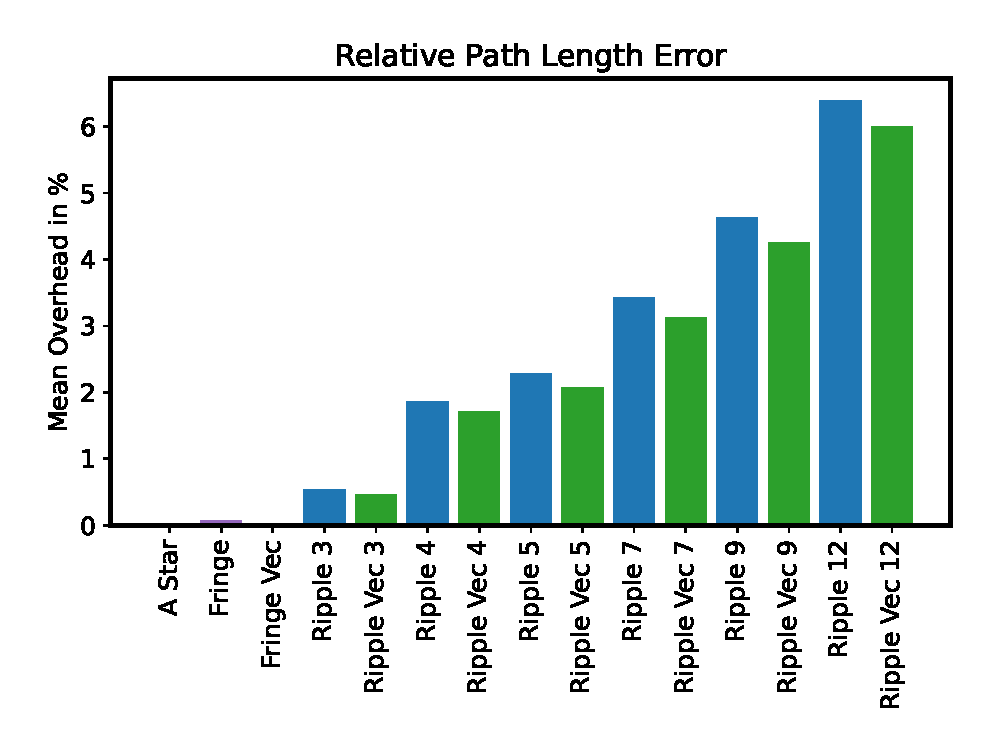
\includegraphics[width=\linewidth]{img/cost_overhead.eps}
    \caption{Mean path cost overhead represented as a percentage of the optimal cost for all benchmark scenarios.}
    \label{fig:cost-overhead}
\end{figure}

\mypar{Consistency}
Lastly, the variance of path length and runtime for each algorithm needs to be assessed. 
As can be seen in \figref{fig:var-time}, adding more threads results in consistently better runtime performance, and surprisingly, PRS runtime was most consistent at very high thread counts.

\begin{figure}[H]
    \centering
    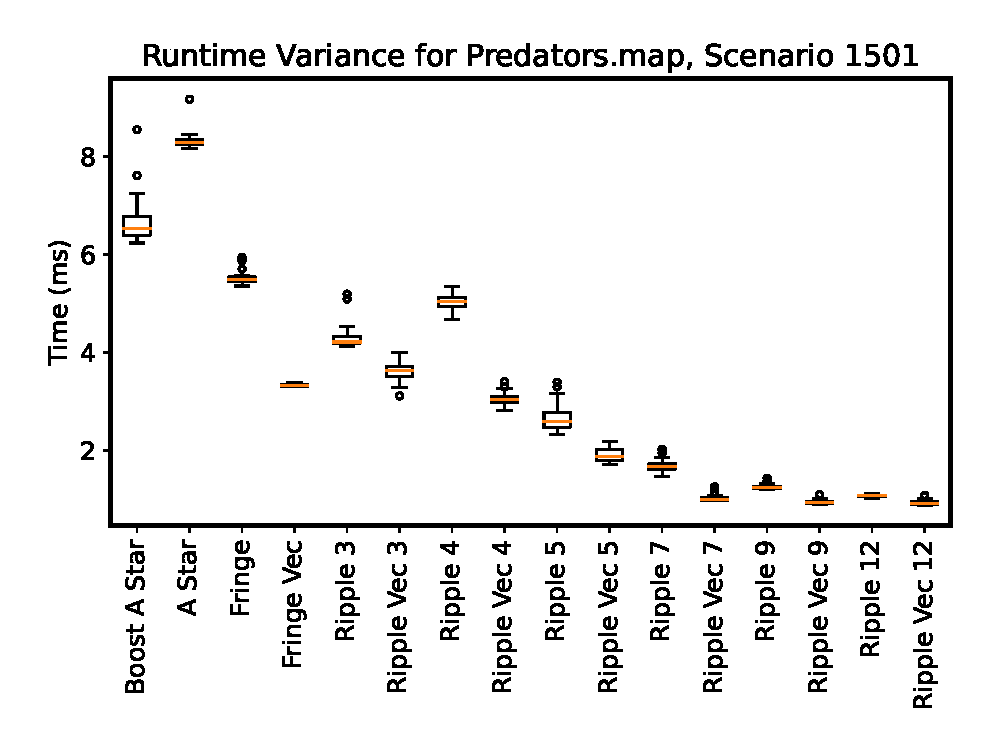
\includegraphics[width=\linewidth]{img/scenario_time.eps}
    \caption{Variability of path length for a representative scenario of the benchmark set, same as used in \figref{fig:ripple_example} and \ref{fig:high}.}
    \label{fig:var-time}
\end{figure}

\noindent Seen in \figref{fig:var-cost}, deterministic search algorithms have zero variance in found path length and PRS length variance increases with the thread count, all as expected.
Over the full run of benchmarks, the variability of each algorithm was low enough in both path length and runtime that further discussion will be omitted, see \figref{fig:var-overall}.
Instead, a decision was made to focus on a hand-picked representative scenario to show consistency in runtime and path quality. 

\begin{figure}[H]
    \centering
    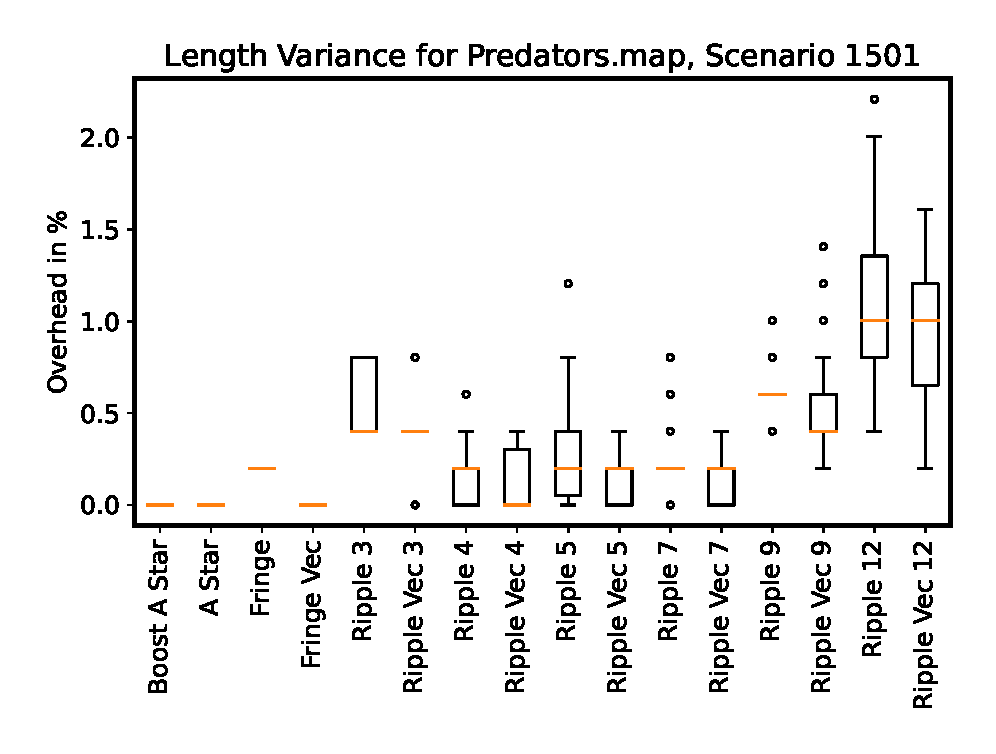
\includegraphics[width=\linewidth]{img/scenario_cost.eps}
    \caption{Variability of path length for a representative scenario of the benchmark set, same as used in \figref{fig:ripple_example} and \ref{fig:high}. The optimal path length is $498$ vertices.}
    \label{fig:var-cost}
\end{figure}

\begin{figure}[h]
    \captionsetup[subfigure]{labelformat=empty}
    \subfloat{
        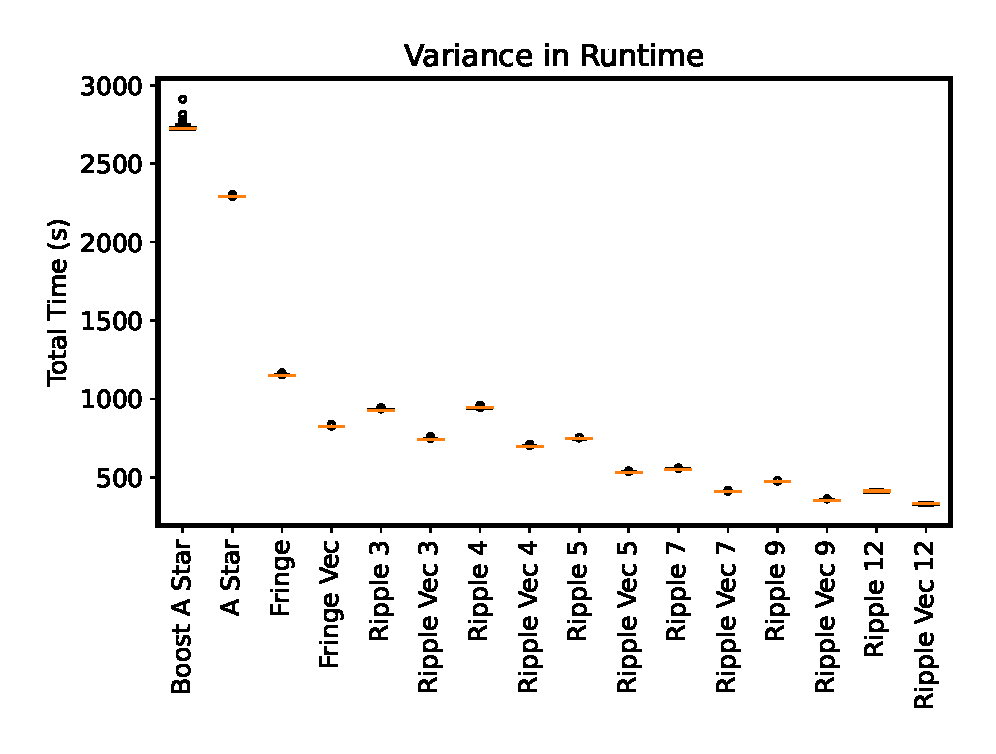
\includegraphics[width=0.22\textwidth]{img/var_time.eps}
    }
 	\hfill
	\subfloat{
        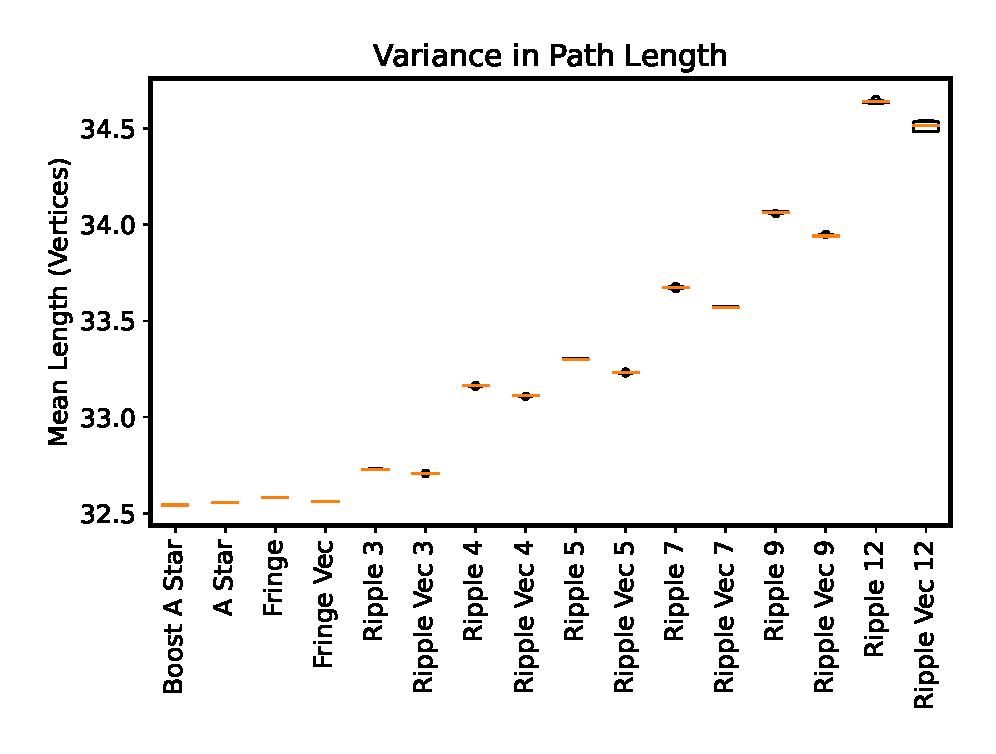
\includegraphics[width=0.22\textwidth]{img/var_cost.eps}
    }
    \caption{(Left) Variability in total runtime over all benchmark scenarios. (Right) Variability in mean path length over all benchmark scenarios.}
    \label{fig:var-overall}
\end{figure}

\section{Conclusion}
In this report, an implementation of the multi-core \textit{Parallel Ripple Search} was described, accompanied by benchmarks against several serial algorithms. 
PRS is able to efficiently utilize multi-core architectures without the need for expensive synchronization primitives such as locks.
It was found that PRS achieves significant speedup with acceptable degradation in path quality. 
PRS serves as a demonstration of how old problems can be re-solved using parallel technologies and architectures fully utilizing the capabilities of modern systems.

\mypar{Future Work}
Within PRS there are many ways the implementation can be tailored and here only a few of them discussed or explained.
In this project, the decision was made to implement the individual search threads using a fringe search in its core loop. 
While this was the serial algorithm that performed best in benchmarks, the work distribution strategy of PRS can be applied to most other pathfinding algorithms.
Future work could investigate different choices for the core algorithm and for the heuristic used, which could lead to better trade-offs between path quality and speed. 
In particular, the heuristic used for the search threads containing the global source or target vertex appeared to be sub-optimal in some cases. An example of this can be seen in \figref{fig:ripple_example}.
Even though only graphs with a grid structure were considered for benchmarking, this implementation is also applicable to general graphs. 
A domain specific application of PRS could optimize certain aspects of the algorithm, tailoring them to the domain and known characteristics of the underlying graphs.
Finally, more sophisticated collision handling could lead to improved path quality. For example, one could remember multiple collisions between distinct pairs of threads and use these to find a lower cost path through the collision graph.



% References should be produced using the bibtex program from suitable
% BiBTeX files (here: bibl_conf). The IEEEbib.bst bibliography
% style file from IEEE produces unsorted bibliography list.
% -------------------------------------------------------------------------
\bibliographystyle{IEEEbib}
\bibliography{bibl_conf}

\end{document}

